\chapter{Разработка приложения реализующего интерполяцию входных данных и ее визуализацию}

\section{Описание функциональности программного обеспечения}

Разработанная программа решает задачи построения цифровых моделей местности с помощью методов интерполяции и непосредственного отображения построенной поверхности в окне приложения. Программное обеспечение в данной работе имеет ряд функций. 

\begin{enumerate} 
  \item[1.] Возможность загрузить текстовый файл с входными значениями для построения поверхности, в формате $X$, $Y$, $Z$, где $X$ -- значение координаты по оси $x$, $Y$ -- значение координаты по оси $y$, $Z$ -- значение точки в этих координатах, все значения разделены пробелом, дробная часть отделяется запятой.
  \item[2.] Возможность выбрать метод интерполяции для построения поверхности, а именно метод интерполяции сплайнами, метод обратно взвешенного расстояния, метод с использованием радиально-базисной функцией.
  \item[3.] Возможность задать размер элемента в метрах для выполнения интерполяции (шаг интерполяции), чем меньше шаг тем более точные значения получаются и цифровая модель местности выглядит более гладко.
  \item[4.] В окне приложения есть два поля для вывода минимального и максимального значений на поверхности и возможность присвоить для этих значений цвета из палитры для отрисовки градиента.
  \item[5.] Возможность визуализации цифровой модели местности с помощью градиента в окне приложения.
  \item[6.] Возможность сохранения итогового файла с интерполированными значениями в текстовом формате.
  
\end{enumerate} 

\section{Архитектура программного обеспечения}

Диаграмма классов (рисунок~\ref{fig:12}) представляет собой визуализацию структуры классов и их отношений в системе. Каждый класс содержит в себе атрибуты и методы, которые определяют их поведение и функциональность. 

\begin{figure}[h!]
    \center
    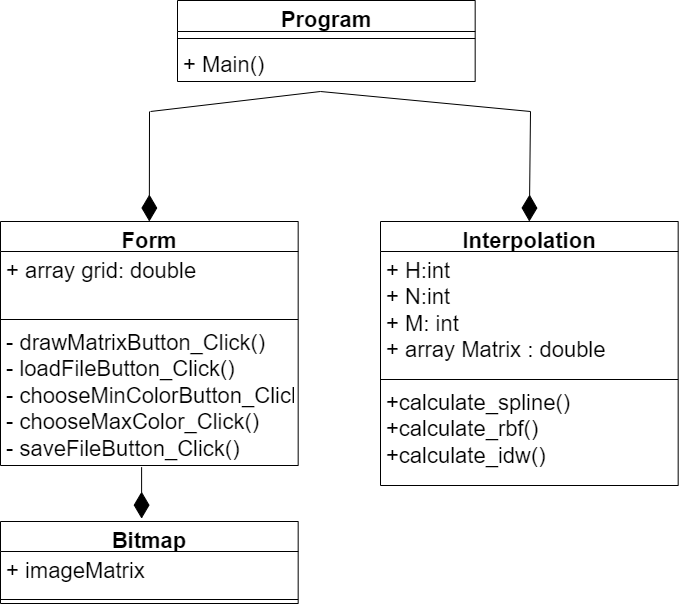
\includegraphics[scale=0.6]{images/diagram class.png}
    \caption{Диаграмма классов спроектированного приложения}
    \label{fig:12}
\end{figure}

Класс Program является основным классом, в котором содержатся такие классы как Form и Interpolation. Отношения между этими классами являются композицией, так как эти классы являются частью класса Program и не могут существовать без него. 

В классе Form содержатся методы для загрузки файла с входными значениями, визуализации проинтерполированной поверхности, выбора цвета минимального и максимального значений и сохранения значений для построенной поверхности. От данного класса идет отношение композиции к классу Bitmap, потому что визуализация поверхности происходит с помощью объекта класса Bitmap и вне класса Form он существовать не будет.

Также класс Interpolation содержит в себе поля и методы необходимые для интерполяции поверхности, в зависимости от выбранного метода интерполяции будет вызываться определенный метод из этого класса. 

Диаграмма вариантов использования (рисунок ~\ref{fig:13}) описывает функциональность системы и ее взаимодействие с пользователем или другими системами. Она показывает различные сценарии использования системы. 

\begin{figure}[h!]
    \center
    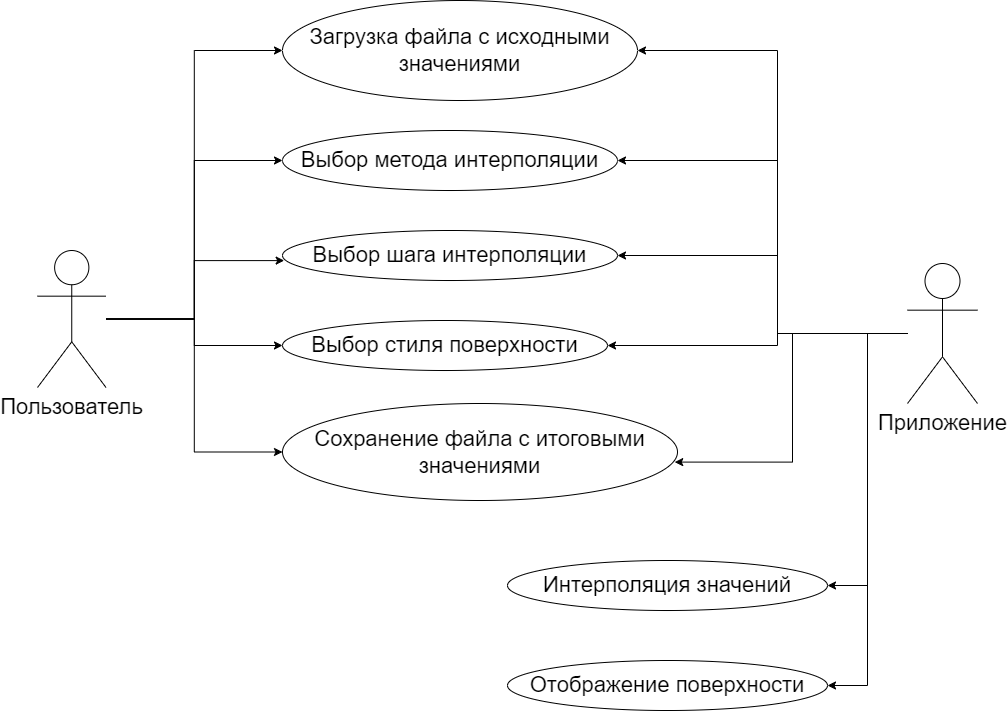
\includegraphics[scale=0.5]{images/Диаграмма вариантов использования.png}
    \caption{Диаграмма вариантов использования спроектированного приложения}
    \label{fig:13}
\end{figure}

Пользователь может загрузить файл с исходными значениями, выбрать метод и шаг интерполяции, выбрать стиль поверхности и запросить сохранение файла с итоговыми значениями. Приложение принимает параметры от пользователя и в зависимости от его запроса интерполирует значения, отображет построенную поверхность или сохраняет файл с итоговыми значениями. Возможности пользователя были определены на основе главного функционала проектируемого приложения.


\section{Используемые технологии и язык программирования}

Разработанное приложение было написано на языке программирования C\#, платформа для разработки и запуска приложений .NET Framework 4.7.2, интерфейс пользователя был выполнен в Windows Forms, средой разработки являлось Microsoft Visual Studio.

Этот язык программирования был выбран, так как он имеет множество плюсов. 

\begin{enumerate} 
  \item[1.] Простой и понятный синтаксис, который делает его легким для изучения и использования.
  \item[2.] Может быть использован для создания приложений для различных платформ, включая Windows, Linux и macOS.
  \item[3.] Имеет встроенные механизмы безопасности, такие как проверка типов и управление памятью, которые помогают предотвратить ошибки и уязвимости.
  \item[4.] Является основным языком программирования для разработки приложений на платформе .NET Framework, что обеспечивает широкий доступ к библиотекам и инструментам.
  \item[5.] Поддерживает объектно-ориентированное программирование, что позволяет разработчикам создавать более модульный и гибкий код.
  \item[6.] Является компилируемым языком программирования, что обеспечивает высокую производительность и быстродействие приложений.
\end{enumerate} 


Данное программное обеспечение могло иметь клиент-серверную архитектуру и работать в браузере для   упрощенного доступа к приложению (нет необходимости скачивать), кроссплатформенности и современных решений для графического интерфейса пользователя, однако так как используемые методы интерполяции могут вызывать высокую нагрузку на центральный процессор, то появляется необходимость использовать строго типизированные языки программирования имеющие высокую оптимизацию при компиляции, что и поспособствовало выбору платформы и языка программирования описанных выше. 

\section{Описание интерфейса программного обеспечения}

Интерфейс программного обеспечения позволяет пользователям взаимодействовать с приложением через наглядные элементы управления, такие как кнопки, поля ввода, выпадающие списки и графическая область (рисунок~\ref{fig:14}).

Пользовательский интерфейс программы состоит из одного окна, логически поделенного на две области каждая из которых предназначена для выполнения определенных задач. Область окна программы в левой части содержит функции для открытия, сохранения и вывода в область отображения данных. Так же есть такие настройки как: выбор метода интерполяции для построения поверхности, настройка цветовой палитры, размер шага интерполяции.

Область окна программы в правой части представляет собой графическую область, в которой отображаются результаты работы программы, а именно цифровая модель местности. В зависимости от выбранных настроек, в этой области могут отображаться различные цифровые модели местности.

Для ввода данных в программу используется кнопка, по нажатию которой открывается рабочая директория из которой можно выбрать текстовый файл с входными значениями. Введение значений вручную не предусматривается.

Интерфейс программы разработан с учетом принципов удобства использования, все элементы управления расположены логически и интуитивно понятно, что позволяет пользователям быстро осваивать программу и использовать ее для построения цифровых моделей местности.

\begin{figure}[h!]
    \center
    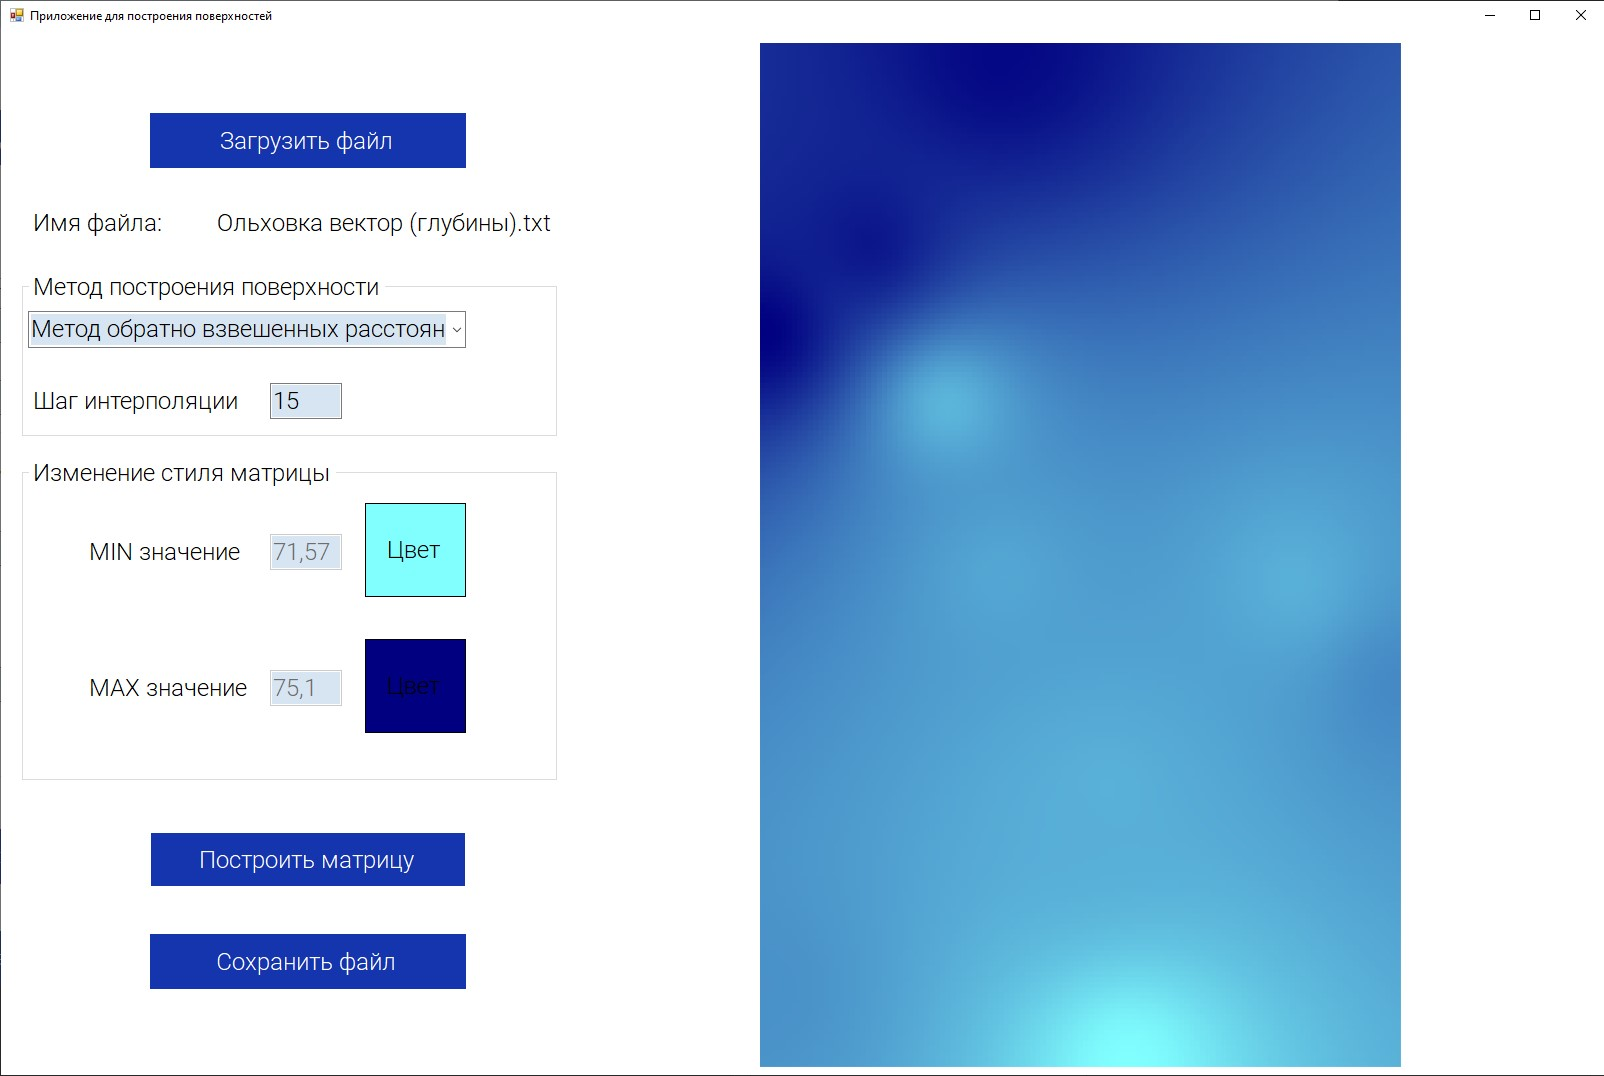
\includegraphics[scale=0.4]{images/Interface.jpg}
    \caption{Интерфейс разработанного приложения}
    \label{fig:14}
\end{figure}

